\chapter{Local maladaptation interacts with expansion load during species range expansions}
\label{chap:expansionload}

\section*{Abstract}

The biotic and abiotic factors that facilitate or hinder species range expansions are many and complex. We examine the impact of two genetic processes and their interaction on fitness at range edges during expansion: local maladaptation resulting from the presence of an environmental gradient, and expansion load resulting from increased genetic drift at the range edge allowing deleterious alleles to reach high frequencies. Our results indicate that the presence of an environmental gradient during range expansion reduces expansion load. On the other hand, increasing expansion load reduces maladaptation at the range edge, which allows marginal populations to be better adapted to their local environment. The fitness reduction caused by both of these processes slows the rate of range expansion, allowing for more genetic rescue than would be expected in the absence of these interactions. This reduction in fitness may have ramifications for species being forced to shift their ranges due to climate change or other anthropogenic changes. If rapidly changing climate requires faster expansion, populations may suffer reduced fitness beyond previous expectations and risk stochastic extinction.

\newpage{}



\section*{Introduction}

%broad intro:
Species range expansion is a complex process that is widely studied in evolutionary biology, ecology, and conservation biology \citep{Chen:2011, Colautti:2013, Hastings:2005, Phillips:2006, Excoffier:2009, Hallatschek:2010}. The array of factors that can contribute to the ability or failure of a species to expand make it difficult to predict when a species will move into novel environments. Many ecological and evolutionary factors are known to affect range expansion, such as dispersal limitation \citep{Hargreaves:2014b, Marsico:2009, Hastings:2005}, species competition \citep{Case:2000, Price:2009,Svenning:2014, Louthan:2015}, or the inability to adapt to new conditions \citep{Polechova:2015, Holt:2011, Angert:2008}. A recently growing field of research has focused on the effects of genetic load accumulated during the expansion process \citep{Excoffier:2009, Hallatschek:2010, Peischl:2013, Peischl:2015, Peischl:2015b}. In particular, the effects of range expansion increasing deleterious variants in human populations that have expanded out of Africa have been widely studied \citep{Henn:2015, Do:2015, Lohmueller:2008}. In this study, we explore the impacts and interactions of heterogeneous selection due to an environmental gradient and the accumulation of deleterious mutations during range expansion.

% range expansions:
Range expansions exhibit an intriguing suite of population genetic processes that can change the course of evolution relative to expectations for stationary growth of populations. Populations at the front edge of a range expansion undergo serial founder events where each new colonization into further territory creates a population bottleneck, leading to reduced genetic diversity in what becomes the new edge population and a primary source of future colonizations. These processes create a persistently reduced effective population size at the range edge, reducing the efficacy of selection and increasing the strength of random genetic drift. This leads to the process of allele surfing \citep{Klopfstein:2006}, whereby a deleterious mutation that arises at the range edge is more likely to drift to high frequency than it otherwise would if it arose in the dense core of the species range. Because selection is weak, these deleterious alleles may have much larger effects than could exist in a population at equilibrium \citep{Peischl:2015}. Allele surfing is the main cause of increased deleterious alleles within recently expanded populations \citep{Excoffier:2009}. The reduction in fitness due to the accumulation of these deleterious alleles is termed the expansion load \citep{Peischl:2013,Peischl:2015}.

% deleterious mutations:
Apart from theoretical predictions, expansion load has been posited as an explanation for the accumulation of deleterious alleles in empirical populations having undergone recent geographic expansions \citep{Karlsson:2014}, in particular for studies of human diseases in populations of Quebec \citep{Scriver:2001, Yotova:2005, Labuda:1997} and Scandinavia \citep{Norio:2003}%check that this ref is appropriate
. A large point of controversy, however, is the likelihood of these deleterious mutations persisting at high frequencies in modern populations. It has only recently been shown that as an expansion proceeds, the distribution of effect sizes can be impacted by deleterious mutations of larger effect rising in frequency \citep{Henn:2015}. Expansion load may thus have the potential for serious repercussions in many species that experience expansions. Understanding the detriment caused by this process may aid in efforts to combat invasive species or in assisted migration. Under the effects of global climate change, more species than ever may be required to move their ranges in order to survive, and if accumulating fitness losses simply due to the expansion process is widespread, populations may be left at higher risk for extinction from stochastic, catastrophic events. %% add something to extend out of human only expansions - talk about glacial recolonizations?

% environmental gradients:
The evolution of populations at the edge of species ranges is unusual in other ways as well. If selective environments vary over space, populations at range edges are likely at least somewhat maladapted to local conditions.  A foundational study by \citet{Kirkpatrick:1997} showed that steep environmental gradients can reduce the ability of a population to expand, because of the failure of the population to adapt to local conditions and migration load caused by dispersal from populations in the core adapted to different conditions. For a population existing within a species range and on a linear environmental gradient, symmetric migration from either adjacent population will contribute alleles that are locally maladaptive, but this balance of immigrant alleles does not change the population mean much from its local optimum. In contrast, at a range edge, immigration comes largely from one direction, causing edge populations to diverge from their local optimum. When migration rates are high enough, the edge population can fail to adapt.  When the environmental gradient is steep enough, the edge populations can go extinct, possibly leading to global extinction of the species as asymmetric migration at the edge continues. Apart from asymmetric migration, steep environmental gradients alone can result in large enough migration load that the species range contracts, potentially to extinction. Further studies \citep{Barton:2001, Polechova:2015} have added additional biological realism (including evolution of genetic variance and effects of genetic drift to models of range expansion), confirming that evolutionary processes alone can form a stable range edge.

% say something about migration load and genetic rescue?


% their interaction and what this study is doing:
It is clear that expansion load can result in reduced fitness of recently expanded populations, and that heterogeneous selection on an environmental gradient can result in local maladaptation of populations at the edge of a species range. The combination of these two effects --- maladaptation from underlying environmental gradients and expansion load from genetic drift of deleterious mutations at range edges --- has not previously been studied. These two evolutionary processes could interact in numerous ways, and a priori we contemplated two contrasting hypotheses for how they may interact. One possibility is that local maladaptation and expansion load may positively interact (i.e., each making the effects of the other more pronounced). This could be expected because both processes are enhanced by the smaller population sizes generated by each of these two forces: expansion load increases because greater drift would cause more deleterious alleles to increase in frequency, and maladaptation worsens because greater drift would eliminate more of the genetic variance needed to respond to local selection. On the other hand, it is possible that expansion load and local maladaptation could negatively interact, with each partially ameliorating the effects of the other. This possibility seems plausible because both expansion load and local maladaptation are reduced by slower range expansion, and each of these forms of load ought to reduce the pace at which ranges expand by reducing fitness of the individuals at the range margin. Expansion load is reduced with slower range expansion because more time allows fit alleles to reach the edge to rescue expansion load, and slower range expansion should allow more time for local populations to adapt to local conditions.

Therefore we have reasonable contrasting hypotheses for how local maladaptation and expansion load may interact to determine the pace of range expansion. We investigate here the role of each of these factors in isolation as well as in combination. Our goal is to employ the most biologically reasonable parameters possible within the realm of our model. Using individual-based simulations on a two dimensional, spatially explicit, and approximately continuous landscape, we compare the reductions in fitness (load) that populations experience during range expansions over a series of environmental gradients and deleterious mutational parameters. These results have implications for the predicted prevalence of expansion load in species across various types of environments and inform our understanding of the complex demographic and genetic processes that occur during range expansions. 


\section*{Methods}


% broad summary of what we modeled:
We model a species range expansion forward in time using the simulation program \textsc{nemo} \citep{Guillaume:2006}. The population undergoes an initial burn-in period to mutation-selection equilibrium, after which the population is allowed to expand across empty landscape. Individuals are monoecious and diploid, possessing both a quantitative trait experiencing stabilizing selection and a set of loci subject to unconditionally deleterious mutations. We compare three different environmental gradients over which expansion occurs, and three different genome-wide deleterious mutation rates. All combinations of parameter values are listed in Table \ref{tab:paramresults}. We ran twenty independent replicates for each of our simulated scenarios.


\subsection*{The Model}

% landscapes
The environmental gradient underlying the landscape changes in only one dimension, along the axis of expansion. We compare three values for the steepness of this gradient, $b$, which defines the change in phenotypic optimum over space: a flat landscape with no gradient ($b = 0.0$), a moderate gradient ($b = 0.0375$), and a strong gradient ($b = 0.375$). On the moderate (shallow) gradient, an average dispersal distance of an individual would result in a loss in fitness of $0.5\%$ if it were perfectly adapted in its natal environment, whereas on the strong (steep) gradient, an average dispersal event would reduce an individual's fitness by $5\%$ given perfect adaptation in its natal environment. Each of these gradients results in a different equilibrium level of migration load in populations.

% landscape and population details - and general model details
We model space explicitly on a $40\times2000$ unit landscape using a modified version of \textsc{nemo} available at \url{https://github.com/kjgilbert/NemoDispersalKernel}. This modification allows a discrete approximation of continuous space. The landscape is divided into 80,000 square units, termed cells, over which a dispersal kernel and breeding window occur, allowing individuals to interact over a much larger spatial scale.  Lifecycle events occur in the order of breeding, dispersal, selection, and then population regulation. Subpopulation regulation enforced a carrying capacity of 6 per cell, but because breeding is not limited to within one cell, the realized neighborhood size as defined by \citet{Wright:1946} is approximately 300 individuals.

%--------- Remi's calculations ---------
%Here is how I calculated it. Note that I used the original formal definition by Wright but in empirical papers, authors seem to playfully use different definitions!
%The "neighbourhood size" is the number of individuals present in the "neighbourhood area", an area where parents can be considered representative of the offspring. The first one to use this term was Wright. In Wright 1945 (page 41). Wright defines the "neighbourhood area" as the circle of $2 \sigma$ of radius, where $\sigma$ is the standard deviation of the migration distance. The "neighbourhood size", is therefore $\pi * n$, where $n$ is the number of individuals in a big square of $2 \sigma$ on a side. 
%In our case $\sigma = 2$ demes for both the leptokurtic and normal distribution and the population per small deme is 6. As a a consequence $n = (2*2)^2 * 6 = 96$ and the "neighbourhood size" is $96 * pi \approx 301.59$ individuals.
%------ End of Remi's calculations ------

Populations were initiated at carrying capacity in the left-most $40\times40$ units of the landscape, which we term the landscape core (Figure \ref{fig:landscape}). After a burn-in period of 15,000 generations, the remaining $40\times1960$ units of the landscape become available, allowing for expansion to occur. We will hereon refer to a 40-unit width of the landscape, across which the environmental optimum is constant (perpendicular to the axis of expansion), as a cross-section.

\begin{figure}[h]
\centering
\makebox[\textwidth]{
        \includegraphics[width=1\linewidth]{Figures/Landscape_Graphic.pdf}}
\caption[~- Landscape graphic.]{Landscape graphic representing an example of the landscape simulated with a grid of units where the burn-in period occurs in the landscape core at the left, expansion proceeds to the right, and any vertical column of units is a cross-section. Actual landscapes were $40\times2000$ units with a $40\times40$ core.}
\label{fig:landscape}
\end{figure}


% breeding
\subsubsection*{Breeding}
Our modified version of \textsc{nemo} creates a breeding window within which individuals may search for a mate within their own cell on the landscape or in nearby cells. Mating probability follows an approximate bivariate Gaussian function which we derive by integrating the probability over each cell within the breeding window. We define the size of this breeding window with the parameter $\sigma_{breed}$, where $f(x,y) \propto \exp{[-(\frac{\Delta x^2}{2\sigma_{breed}^2}+\frac{\Delta y^2}{2\sigma_{breed}^2})]}$ gives the distance traveled to search for a mate in each dimension of the landscape. $\sigma_{breed}$ was held constant at $0.5$ landscape units. The maximum searchable distance was restricted to $4\sigma_{breed}$ with probabilities renormalized to correct for this truncation. This resulted in a two-dimensional breeding window where an individual's focal cell is the most likely source of a mate and the 12 surrounding cells could be searched for a mate with decreasing probability. This breeding dispersal kernel describes the relative probability of each individual within the possible breeding window being chosen as the male parent for a given offspring. When no other individuals are present within the breeding window, an individual self-fertilizes. This will most often happen at the expanding range edge where population densities are lowest and mimics the ability of many plant species to self under conditions of pollen limitation \citep{Hargreaves:2014}. Each female's fecundity was drawn from a Poisson distribution with mean 7 to determine the number of mating events. 

\subsubsection*{Dispersal}
% dispersal
We modeled dispersal for most simulations according to an approximate bivariate Gaussian kernel, similarly to the breeding kernel: $f(x,y) \propto \exp{[-(\frac{\Delta x^2}{2\sigma_{disperse}^2}+\frac{\Delta y^2}{2\sigma_{disperse}^2})]}$. The dispersal kernel gives the forward migration probabilities for offspring to disperse to a given patch. Unlike the breeding kernel, the maximum dispersal distance was capped at a distance of $8\sigma_{disperse}$. $\sigma_{disperse}$ for the Gaussian dispersal kernel was set to equal two landscape units. We also simulated a leptokurtic kernel, to test the effects of rare, long-distance dispersal events. The leptokurtic dispersal kernel was a mixture distribution created from a weighted sum of two different Gaussian kernels \citep{Ibrahim:1996} with the same average dispersal distance as the Gaussian kernel and a total kurtosis of 10. This value of kurtosis is not unrealistic for long-distance dispersal in many species \citep{Guttal:2011, Lowe:2009, Skalski:2000}. The first distribution used $\sigma_{disperse}$ equal to 1.5 with a weighting of 0.89, while the second used $\sigma_{disperse}$ of 5.5 and a weighting of 0.11. The leptokurtic kernel was cut off to have the same maximum dispersal distance, which in both cases meant an individual could at most disperse 16 units in any one direction from its natal cell. Borders of the $40\times2000$ landscape were absorbing, so any individual migrating beyond the edge was removed. R code for calculating and discretizing the dispersal and breeding kernels is available in a wrapper package written for \textsc{nemo}, \textsc{aNEMOne}, available at: \url{https://github.com/kjgilbert/aNEMOne}.


\subsubsection*{Genetics}
% paragraph on quanti traits & selection
We modeled a genetic architecture where 100 quantitative trait loci and 1000 loci subject to unconditionally deleterious mutations were randomly and independently placed on the genome for each simulation. Each genome consisted of ten chromosomes of 100 cM each. We selected realistic mutational parameters for these loci as follows.

The quantitative trait, $z$, was controlled by 100 additive loci. Each allele at these loci can take any real value. The evolution of this trait under stabilizing selection depends on the mutational variance, $V_M$, and the inverse strength of stabilizing selection on the trait, $\omega^2$. These properties have been empirically estimated for a number of traits, along with the corresponding environmental variances, $V_E$. For our model we set $V_M$ and $\omega^2$ relative to the same arbitrary $V_E$ value ($V_E = 1$). There is evidence that $\omega^2 \approx 5 V_P$ on average (where $V_P$ is the phenotypic trait variance; \citet{Kingsolver:2001, Johnson:2005}). The relationship between $V_P$ and $V_E$ can be expressed in terms of heritability, $h^2 = 1 - \frac{V_E}{V_P}$, and we can therefore write $\omega^2 \approx \frac{5V_E}{1 - h^2}$. Given $V_E = 1$ and a typical heritability of $h^2 \approx \frac{1}{3}$ \citep{Mousseau:1987, Houle:1992}, we set $\omega^2 = 7.5$.  

Most reported values of $\frac{V_M}{V_E}$ are in the range $10^{-4}$ to $10^{-3}$ \citep{Houle:1996}. $V_M$ depends on the genome-wide rate of mutations affecting the trait, $U_z$, and the expected squared effect of a mutation on the trait, $E[\alpha^2]$, where $V_m = U_z E[\alpha^2]$. If mutational effects are Gaussian with $E[\alpha] = 0$, then $E[\alpha^2] = V[\alpha]$, the variance of mutational effects on the trait. These components are difficult to estimate, but according to one theoretical approach we expect $V_P - V_E = 4 U_z \omega^2$ \citep{Turelli:1984, Charlesworth:2010}. Given the parameters above, this implies $U_z \approx 0.02$, similar to some direct estimates \citep{Lynch:1998}. In our simulations we used 100 quantitative trait loci, with a mutation rate per locus of $1\times10^{-4}$, giving a diploid mutation rate, $U_z$, of $0.02$. We further assumed $V[\alpha] = 0.02$ (i.e., mutational effects on $z$ are drawn from a normal distribution with mean 0 and variance 0.02), giving a conservative value for $V_M$ of $4\times10^{-4}$.

In this model an individual's trait value is given by the sum of allelic effects across all quantitative trait loci, with no dominance. Alleles are continuous, such that a mutation's effect is added to the existing allelic value. The component of fitness (survivorship) for the quantitative trait value $z$ is $w_z = exp[-\frac{(z-z_{opt})^2}{2\omega^2}]$, where $z_{opt}$ is the optimal trait value for the given location on the landscape. At the start of the burn-in, all individuals were initiated with $z$ equal to the mean $z_{opt}$ of the burn-in area (core). 

% add this in as a section distinguisher?  \paragraph{Deleterious Mutations}
We also modeled 1000 bi-allelic loci subject to unconditionally deleterious mutations. We considered genome-wide diploid deleterious mutation rates, $U_D$, of 0.1 and 1.0 in order to encompass probable rates for a variety of taxa, including \emph{Drosophila melanogaster} \citep{Haag:2007}, \emph{Caenorhabditis elegans} \citep{Denver:2004}, \emph{Arabidopsis thaliana} \citep{Shaw:2000}, \emph{Amsinckia sp.} \citep{Schoen:2005}, and possibly non-human endothermic vertebrates \citep{Baer:2007}. However, we note that in humans $U_D$ likely exceeds 1.0 \citep{Keightley:2012}, and $U_D$ is likely less than 0.1 in many other organisms \citep{Baer:2007, Halligan:2009}. We also included a treatment where deleterious mutations were absent ($U_D = 0.0$). Deleterious mutation rates per haploid locus were thus $0$, $5\times10^{-5}$, and $5\times10^{-4}$, and we allowed for back-mutation at rates of $0$, $5\times10^{-7}$, and $5\times10^{-6}$, respectively. Once mutated, a locus could not further mutate and the only possible change would be due to a back-mutation. These 1000 loci do not accurately portray the number of possible loci in biological systems, but are instead an approximation required by simulation. By matching our genome-wide mutation rates to realistic values, each of these loci is more representative of a region of the genome within which a deleterious mutation may arise. Thus, for the distribution of effects we use, described below, small effect mutations may be approaching saturation, but because these small effect loci do not contribute substantially to fitness reductions, this lack of realism in terms of the number of loci is not detrimental to our model and its results. 

Though the true distribution of mutational fitness effects is empirically difficult to measure and may be complex, there is evidence that most mutations have small effects on fitness, and rare mutations have large effects on fitness \citep{Eyre:2007}. We modeled the homozygous fitness effects ($s$) of deleterious mutations using a leptokurtic gamma distribution with mean $0.01$ and shape $0.3$, such that most mutations have $s < 1\%$ \citep{Keightley:1994}. The mutational effect of each locus was drawn from this distribution at the start of each independent simulation run and remained constant throughout the run.

We modeled the dominance coefficient, $h$, of deleterious allele $i$ as $h_i = exp[-51.1 s_i]/2$. This means that $h$ approaches 0.5 (additivity) as $s$ approaches $0$, and $h$ approaches $0$ (complete recessivity) as $s$ approaches $1$. Given these parameters, %our specified $\bar{h} = 0.3$ results in a realized 
$E[h] \approx 0.37$ and $E[hs] \approx 1.4\times10^{-3}$. This relationship is more realistic than a constant $h$, and captures some of the coarse patterns thought to occur in the relationship between $h$ and $s$ \citep{Agrawal:2011}. Finally, we also included a class of deleterious mutations with $s = 1$ and $h = 0$, i.e., recessive lethals, and assumed that 3\% of deleterious mutations fall into this class to match the genome-wide rate typically observed in \emph{D. melanogaster} \citep{Fry:1999}.


\subsubsection*{Mimicking Mutation Load} % get rid of the subsection, or change it's name to something better
We compared an additional parameter set to the core set described above in order to disentangle the effects of mutation load and expansion load. When populations are at mutation-selection balance, the reduction in fitness due to deleterious mutations is termed the mutation load. During range expansion, the deleterious mutations can increase due to genetic drift during the expansion process. This excess load beyond mutation load is termed the expansion load. To mimic the presence of mutation load only, without expansion load, we altered individual fecundity to reduce realized fitness to a level that matches the mutation load measured in the range core, which has not undergone expansion, for each of our scenarios of $U_D = 0.1$ and $U_D = 1.0$. This was only done for the cases of Gaussian dispersal. We calculated the equilibrium fitness due only to deleterious mutations in the core landscape populations and reduced mean fecundity to recreate this same realized fitness. Mean fecundity in the case matched to $U_D = 0.1$ was approximately 6.475 %6.4749923
and approximately 3.721 %3.7210544.
for the $U_D = 1.0$ case.
% how many sig figs do we want on those numbers? these are the exact ones I put into Nemo



\subsection*{Analyses}
We assess the impact of expansion over an environmental gradient and in the presence of deleterious mutation both independently and in combination. We quantify two measures from the results of simulations: the speed of range expansion and mean fitness. We partition fitness into each of its contributing components, $w_z$ for the quantitative trait and $w_D$ for the deleterious alleles. 

We use a single landscape cross section as the range edge in order to track the expanding front. The speed of expansion measures the number of cross sections over which this edge cross section travels per generation. This edge was defined as the first cross section away from the core at which population size is at 50\% of the core's equilibrium population size. Speed of expansion is a measure of the distance traveled over the landscape from the end of the burn-in until reaching the second to last landscape cross section, divided by the time taken to do so.

To examine fitness at the range edge we defined a larger region of individuals than the cross section used to measure speed of expansion. We defined this range edge to contain all individuals present within the cross section used to measure expansion speed plus all individuals present in cross sections extending rightward, including all individuals until empty landscape is reached. Expansion load measured the excess load that accumulated at the range edge beyond mutation load, calculated as $1 - \frac{edge ~ w_D}{core ~ w_D}$.

Because expansion proceeded at different rates in different scenarios, to create an equivalent comparison of fitness on the landscape we measured populations at the latest recorded point in the simulations before any individuals had dispersed into the last $40\times20$ units of the landscape. Since individuals can at most disperse 16 units, this prevented edge effects potentially encountered upon filling the landscape from altering our results. We averaged population sizes and fitness within cross-sections of the landscape, as we saw no major variation on this axis. 


\section*{Results}

\subsection*{Expansion Speed}
% what are these effects on expansion speed? 
No parameter combinations that we investigated ever led to the formation of a stable range edge. However, the rate at which populations expanded across the landscape was impacted by the presence of heterogeneous selection from the environmental gradient and deleterious mutations. Steeper environmental gradients slowed the speed of expansion (Figure \ref{fig:speed}). Leptokurtic dispersal kernels resulted in faster expansion over the landscape, particularly in the absence of an environmental gradient where expansion speed was 66\% to 76\% greater for leptokurtic dispersal. Increasing the deleterious genomic mutation rate slightly but significantly decreased the speed of expansion (ANOVA $F_{2,358} = 3749.5$,  p $< 0.001$). Steepness of the environmental gradient had large effects on slowing the speed of expansion. The difference between no gradient and the steep gradient slowed expansion in the Gaussian dispersal cases to 20-23\% in the presence of the steep gradient.

\begin{figure}[h]
\centering
\makebox[\textwidth]{
        \includegraphics[width=0.8\linewidth]{Figures/expansion_speed.pdf}}
\caption[~- Average speed of expansion.]{Average speed of expansion across scenarios, measured as the number of landscape cross sections colonized per generation. Circles indicate Gaussian dispersal kernels while triangles indicate leptokurtic dispersal kernels. Dashed lines indicates fecundity-adjusted simulations which replicate the loss in realized fitness due to mutation load, but lack expansion load because no deleterious alleles are present. These refer only to Gaussian dispersal kernels. Error bars indicate 95\% confidence intervals.}
\label{fig:speed}
\end{figure}




\subsection*{Fitness and Load}

In general, the presence of heterogeneous selection or the presence of deleterious mutations both reduced mean fitness in the core and edge, as expected. Furthermore, fitness at the expanding edge was always reduced relative to the core of the species range (Figure \ref{fig:fitness}). The quantitative fitness component, $\bar{w}_z$, in the core was nearly identical across $U_D$ cases and ranged from 0.87 to 0.93 (Table \ref{tab:paramresults}). Fitness reduction at the edge for the quantitative trait only occurred in the presence of an environmental gradient and ranged from a $25-77\%$ reduction in $\bar{w}_z$ at the edge relative to the core. The most severe fitness loss at a range edge was for $U_D = 0$ on the steep gradient ($b = 0.375$) where edge $\bar{w}_z$ was reduced by $22.9\%$ relative to the core.

Fitness for deleterious alleles, $\bar{w}_D$, experienced in the range core reflects the equilibrium mutation load reached in the respective $U_D$ cases. For  $U_D = 0.1$, core $\bar{w}_D$ was $0.92$, while for $U_D = 1$, core $\bar{w}_D$ was $0.53$. Edge $\bar{w}_D$ ranged from $0.80-0.89$ for $U_D = 0.1$ and from $0.32-0.44$ for $U_D = 1$. Table \ref{tab:paramresults} reports all fitness values for the respective scenarios simulated.


\begin{figure}[h]
\centering
\makebox[\textwidth]{
        \includegraphics[width=1.2\linewidth]{Figures/core_edge_fitness.pdf}}
\caption[~- Average core and edge fitness.]{Average core and edge fitness components for quantitative trait and deleterious alleles. Dashed lines indicate fecundity-adjusted simulations which replicate the loss in realized fitness due to mutation load, but lack expansion load because no deleterious alleles are present. Error bars indicate 95\% confidence intervals.}
\label{fig:fitness}
\end{figure}


% is there load and how much
Expansion load for our parameter sets causes a 39\% reduction in fitness at its worst, while at its weakest results in a 3.5\% decrease in fitness (Figure \ref{fig:load}). % this part goes below when talking about the interaction: "We find that expansion load is greatest in the absence of an environmental gradient (Figure \ref{fig:load}). The presence of any environmental gradient significantly reduces expansion load. This effect is greatest on the steepest gradient, where in the case of $U_D = 1$, there is a 45.7\% reduction in expansion load relative to the case of no gradient. In the case of $U_D = 0.1$, the load is reduced by the steepest gradient by 26.6\%." 
Across the two $U_D$ cases, on no gradient, $U_D = 1$ has a 2.95-fold increase in expansion load over the case of $U_D = 0.1$, while on the steepest gradient this change in $U_D$ resulted in a 5.1-fold increase in expansion load.

\begin{figure}[h]
\centering
\makebox[\textwidth]{
        \includegraphics[width=0.5\linewidth]{Figures/expansion_load.pdf}}
\caption[~- Average expansion load.]{Average expansion load across all combinations of environmental gradients and genome-wide deleterious mutation rates. Error bars indicate 95\% confidence intervals.}
\label{fig:load}
\end{figure}


Since leptokurtic dispersal only showed meaningful differences for expansion speed, and not for fitness, those results are presented in supplemental figure \color{red}Sn\color{black}. Supplemental figure \color{red}Sn \color{black} presents detailed results on recovery rates for populations after the expansion process has finished. Furthermore, time-lapse GIFs of fitness and population size across the entire landscape can be seen in supplemental figures \color{red}Sn-Sn\color{black}.


% is amount of migration load/lack of local adaptation impacted by expansion load
\subsection*{Interaction of Expansion Load and Heterogeneous Selection}
We next investigate how each individual component of fitness is affected by reduced fitness in the other component. We examine the impact of expansion load on the level of local maladaptation in populations and alternatively if local maladaptation affects the degree of expansion load. First, does the presence of expansion load increase or decrease the amount of adaptation exhibited in the quantitative trait. We find that an increase in load due to deleterious alleles improves the level of adaptation to the local environment (Figure \ref{fig:fitness}a). This becomes clear when we consider the fecundity-adjustment simulations that lack the presence of expansion load. Within a given value of environmental gradient, $w_z$ increases when only the effects of mutation load are present (fecundity-adjusted runs) and increases even further in the presence of both mutation load and expansion load  ($U_D = 0.1$ and $U_D = 1$). The largest increase in quantitative trait fitness occurs on the weak gradient ($b = 0.0375$) between $U_D = 0$ and $U_D = 1$, where the presence of mutation load leads to a $30\%$ improvement in $w_z$ on average, and the presence of mutation and expansion load together increase $w_z$ by $70\%$. 

% is amount of expansion load impacted by migration load/lack of local adaptation
Second, we find that the severity of expansion load is partially mitigated by the presence of an environmental gradient. We find that expansion load is greatest in the absence of an environmental gradient (Figure \ref{fig:load}). The presence of any environmental gradient significantly reduces expansion load. For a given$U_D$ value, expansion load decreases with increasing gradient steepness. In the case of $U_D = 1$, there is a $45.7\%$ reduction in expansion load from the no gradient to the steepest gradient. In the case of $U_D = 0.1$, expansion load is reduced by the steepest gradient by 26.6\% compared to the case with no environmental gradient. 


\subsection*{Loci Contributing to Expansion Load}
% what is the mechanism of expansion load (effect sizes)
We investigated the details of deleterious mutations accumulating on the expanding population front. Deleterious mutations were binned by effect size into 40 quantiles based on the underlying gamma distribution of homozygous effects. We examined the distribution of alleles contributing to expansion load across cases of $U_D$ and $b$. For $U_D = 1$, the majority of expansion load is due to alleles of intermediate effect (Figure \ref{fig:loci}b). On the steep gradient ($b = 0.375$), there is less load overall due to each locus, but a more constant value across loci of both intermediate and large effect. On the moderate gradient and with no gradient, there are fewer large effect alleles contributing to load relative to the strong gradient, but also many more intermediate-sized alleles contributing to more overall load. For $U_D = 0.1$ (Figure \ref{fig:loci}a), there is less overall load, so lower averages within most ranges of allelic effect size, however we see an inflation of larger effect alleles above that seen for the $U_D= 1$ case in the absence of an environmental gradient.

\begin{figure}[H]
\centering
\makebox[\textwidth]{
        \includegraphics[width=0.9\linewidth]{Figures/load_locibinned.pdf}}
\caption[~- Average expansion load per locus.]{Average expansion load per locus at the range edge. Loci are binned into quantiles drawn from our modeled gamma distribution, shown by the histogram of loci density. Average load per locus is then calculated for each of these bins and plotted for each value of the environmental gradient}
\label{fig:loci}
\end{figure}

There are very few loci present in these larger effect size classes, yet they still contribute largely to expansion load. As can be seen in Figure \ref{fig:allfreqs}, some of these larger effect loci have fixed at the range edge. The effect of surfing which contributes to the fixation of these larger effect alleles can be seen in animation over time with supplemental figure \color{red}XX\color{black}, where recovery from fixation follows behind the expanding wave front.

%%%%%				%%%%%			%%%%%			%%%%%			%%%%%			%%%%%			%%%%%			%%%%%***********	
\begin{figure}[h]%%%%%			 change to the figure with the orange line highlighting the one locus										%%%%%***********	
\centering
\makebox[\textwidth]{
        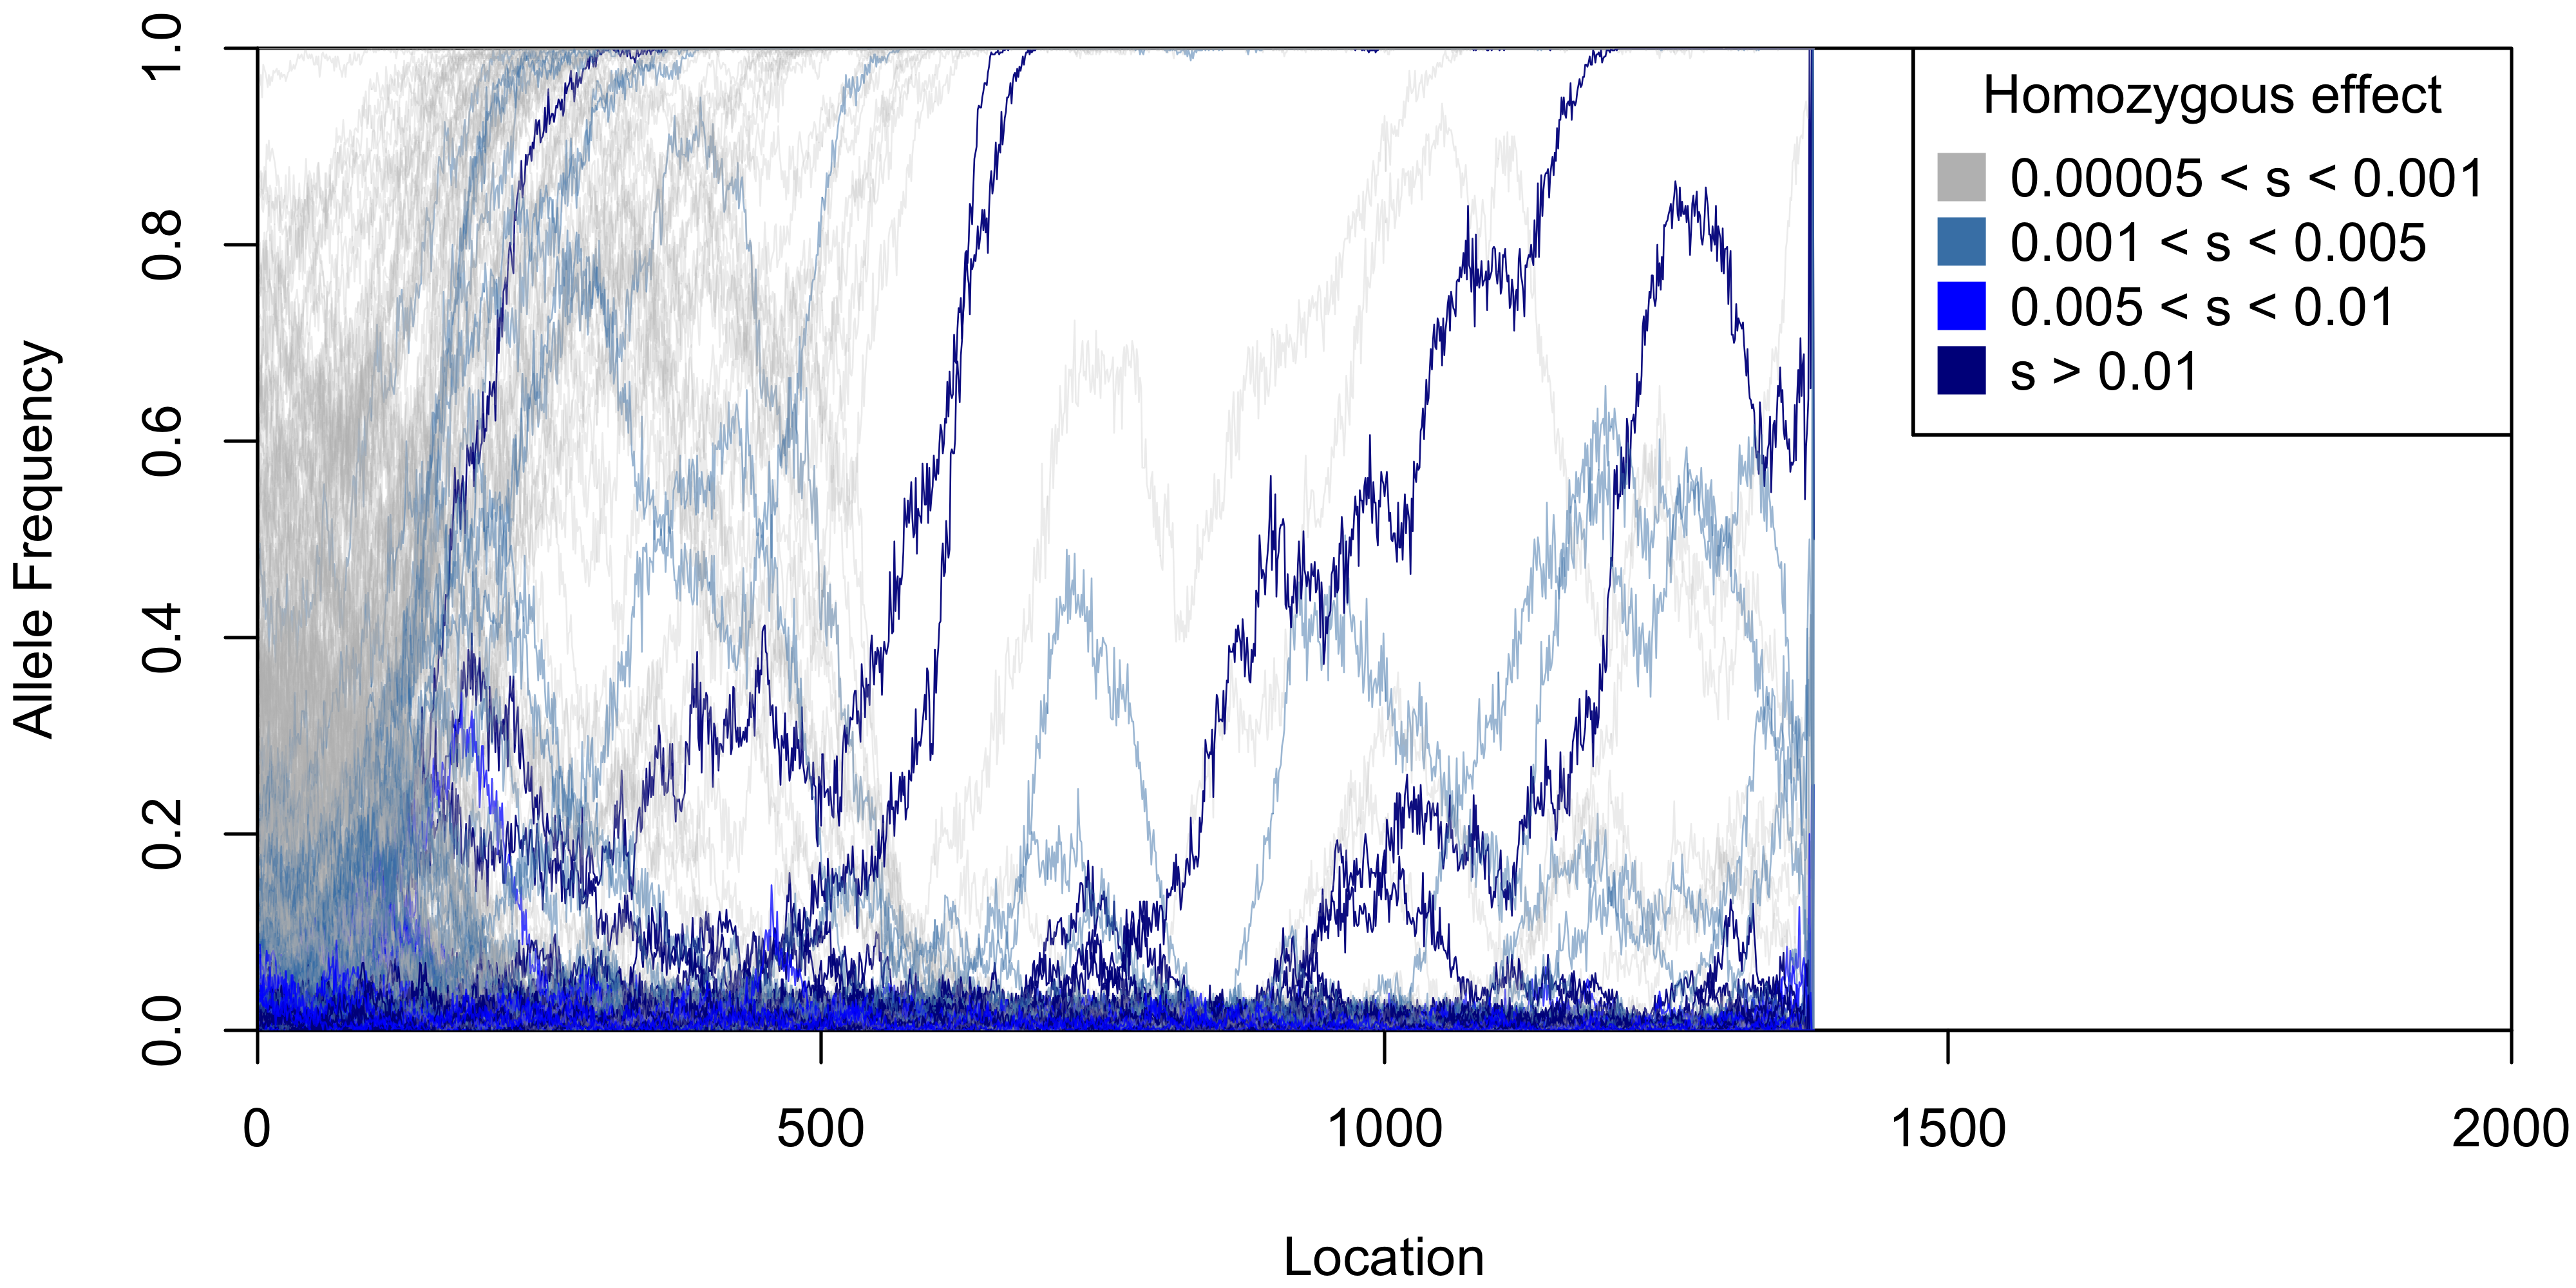
\includegraphics[width=0.9\linewidth]{Figures/example_allfreqs.png}}
\caption[~- Deleterious allele frequencies across the landscape.]{Deleterious allele frequencies across the landscape, binned into classes of homozygote effect size, \emph{s}. This example is at 250 generations after burn-in for the case of a leptokurtic dispersal kernel, $U_D = 0.1$ and $b = 0$. This example was not randomly chosen, but selected to show that large effect loci can locally fix under these conditions. The locus indicated by the thickest line has an effect size of \color{red}XXX\color{black}.}
\label{fig:allfreqs}
\end{figure}

% recovery rates in suppmat




\begin{table}[h]
\centering \footnotesize
\caption[Fitness and expansion speed results per scenario parameter combinations]{Fitness and expansion speed results per scenario parameter combinations. Expansion speeds are shown +/- 1 standard error and fitness measures are shown at the core and the edge.}
\label{tab:paramresults}
\begin{tabular}{p{0.08\textwidth}|p{0.1\textwidth}|p{0.1\textwidth}|p{0.15\textwidth}|p{0.1\textwidth}|p{0.1\textwidth}|p{0.1\textwidth}}
Environ- mental  		& Genomic Deleterious 	& Dispersal Kernel	& Mean Expansion Speed& Total $\bar{w}$	& Quantitative Trait $\bar{w}_z$	& Deleterious Loci $\bar{w}_D$ \\
Gradient (\emph{b})		& Mutation Rate ($U_D$)	&	  			&  			&	\tiny{Core/Edge}	&	\tiny{Core/Edge}				&	\tiny{Core/Edge}	\\ \hline \hline
0.0                       	&	0.0	& Gaussian         &	3.741 +/- 0.005	&	0.932/0.932	&	0.932/0.932	&	1/1	\\
0.0375                    	&	0.0	& Gaussian         &	2.314 +/- 0.011	&	0.929/0.399	&	0.929/0.399	&	1/1	\\
0.375                     	&	0.0	& Gaussian         &	0.756 +/- 0.003	&	0.870/0.199	&	0.870/0.199	&	1/1	\\ \hline
0.0                       	&	0.1	& Gaussian         &	3.559 +/- 0.008	&	0.863/0.748	&	0.933/0.933	&	0.925/0.802	\\
0.0375                    	&	0.1	& Gaussian         &	2.283 +/- 0.011	&	0.859/0.390	&	0.929/0.461	&	0.924/0.845	\\
0.375                     	&	0.1	& Gaussian         &	0.744 +/- 0.002	&	0.804/0.193	&	0.870/0.217	&	0.924/0.891	\\ \hline
0.0                       	&	1.0	& Gaussian         &	2.285 +/- 0.014	&	0.496/0.306	&	0.933/0.945	&	0.532/0.323	\\
0.0375                    	&	1.0	& Gaussian         &	1.991 +/- 0.011	&	0.494/0.268	&	0.929/0.694	&	0.532/0.387	\\
0.375                     	&	1.0	& Gaussian         &	0.595 +/- 0.002	&	0.463/0.160	&	0.870/0.366	&	0.532/0.437	\\ \hline
0.0                       	&	0.0	& Leptokurtic      &	5.689 +/- 0.010	&	0.933/0.929	&	0.933/0.929	&	1/1	\\
0.0375                    	&	0.0	& Leptokurtic      &	2.695 +/- 0.014	&	0.929/0.369	&	0.929/0.369	&	1/1	\\
0.375                     	&	0.0	& Leptokurtic      &	0.736 +/- 0.002	&	0.871/0.183	&	0.871/0.183	&	1/1	\\ \hline
0.0                       	&	0.1	& Leptokurtic      &	5.355 +/- 0.030	&	0.862/0.770	&	0.933/0.936	&	0.924/0.823	\\
0.0375                    	&	0.1	& Leptokurtic      &	2.637 +/- 0.019	&	0.859/0.360	&	0.929/0.420	&	0.924/0.858	\\
0.375                     	&	0.1	& Leptokurtic      &	0.721 +/- 0.002	&	0.803/0.181	&	0.870/0.206	&	0.923/0.881	\\ \hline
0.0                       	&	1.0	& Leptokurtic      &	3.377 +/- 0.045	&	0.498/0.283	&	0.933/0.938	&	0.534/0.302	\\
0.0375                    	&	1.0	& Leptokurtic      &	2.285 +/- 0.014	&	0.496/0.249	&	0.929/0.644	&	0.534/0.388	\\
0.375                     	&	1.0	& Leptokurtic      &	0.577 +/- 0.004	&	0.463/0.162	&	0.870/0.367	&	0.532/0.442	\\ \hline
\end{tabular}
\end{table}







%% add mike's point to discussion - in addition to the quanti trait redicing fitness and slowing expansion therefore reducing load, the same is true for more delet loci, i.e. load calcualted from one delet mut and multiplied up to more would overestimate the actual realized load

\section*{Discussion}


%broadly start discussion for where our study fits into the literature of this field
%why no range limits are found
%compare to polechova and barton 2015
%could bring in relation to bridle et al 2010

Range expansions are unique demographic events that lead to an interesting suite of population genetic processes. These processes have been widely studied, yet examining the combination of both an environmental gradient over which expansion occurs and deleterious mutations that can contribute to expansion load has not previously been investigated. We found that under biologically realistic conditions, both expansion load and the process of adapting to an environmental gradient slow range expansion and lower the fitness of expanding populations. Previous theoretical studies focusing independently on either the effects of expansion load or the process of adaptation on an environmental gradient predicted reduced fitness at the range edge. We find that these factors interact, so that the load at the range edge is not as great as would be expected by a simple combination of the two. This interaction is relevant to studies of expansion load and is important for  predicting the fate of populations undergoing expansions due to natural phenomena or human-induced climate change [\color{red}citation for range shifts under climate change?\color{black}]. 

Our results corroborate previous studies, showing that expansion load accumulates during a species range expansion. The amount of expansion load that we observe is, however, lower than in previous theoretical studies. \citet{Peischl:2013} reported a load of approximately $75\%$ under a soft selection model. Under such conditions, local competition allows greater load to accumulate. Under a hard selection model when fitness is absolute, limiting the expansion load that can accumulate, \citet{Peischl:2015} found an approximate expansion load of $66\%$. Though our simulations also employ hard selection, there are multiple differences in parameter choices and model designs that contribute to the different amounts of load realized. 

The degree of expansion load interacts with many biological factors. Our choice of fecundity greatly impacts the speed at which populations expand across the landscape. Simulations with fecundity set to $3.5$ (data not shown) instead of $7$ showed much less expansion load and higher fitness levels in edge populations. Thus, increasing fecundity allows populations to persist at lower mean fitness and thus accumulate more load. \citep{Peischl:2013} also showed that one- versus two-dimensional models can yield slight differences in results for fitness reductions. 

We find an interesting interaction of the presence of an environmental gradient with the presence of deleterious mutations in our simulations. As expected, this load is higher with more mutational input. Perhaps unexpectedly, however, the greatest expansion load ($39\%$) occurred in the absence of an environmental gradient. Rather than combining additively to further reduce fitness in edge populations, these factors instead interact to reduce load at the range edge. Steeper environmental gradients lead to reduced deleterious mutation load, and higher deleterious mutation rates lead to higher fitness associated with local adaptation to the environment.

We attribute these results to the impact that each form of load has on reducing population fitness and thus the speed of expansion. Expansion across an environmental gradient is more difficult because local adaptation is impeded by migrants creating an influx of maladaptive alleles \citep{Kirkpatrick:1997, Barton:2001, Polechova:2015}. This factor alone can reduce fitness at the range edge, in particular, due to the asymmetry of migration at a range edge where all migrants necessarily come from the core \citep{Kirkpatrick:1997}. As the gradient steepens and increases the difficulty of local adaptation, fitness is decreased and the speed of expansion slows. This time taken for local adaptation is key to the alleviation of expansion load because it provides increased time for genetic rescue and recovery from expansion load. When expansion is slowed, more migrants from the dense core can reach the range edge, and population sizes can recover more quickly.

Populations expanding in the absence of a gradient spread the fastest, as there is no difficulty in local adaptation. This speed of expansion exacerbates the reduced population sizes on the expanding front, further reducing the efficacy of selection at the range edge, and allowing the accumulation of more detrimental mutations. Faster expansion reduces time for recovery to occur from the core of the species range because fewer migrants will be able to successfully reach the expanding front. In a manner analogous to the interaction we present between adaptation of a quantitative trait and the presence of deleterious alleles, this effect would likewise have implications for 1-locus models of expansion load whereby it would be incorrect to assume an additive buildup of load when introducing more loci to a model.


%why kurtotic isn't a thing
Somewhat surprisingly, we found no effect of the shape of the dispersal kernel on the level of local maladaptation or expansion load. Increased long distance dispersal with the leptokurtic dispersal kernel did lead to faster range expansions, but this effect was only notable on a shallow or no environmental gradient. These differences in speed were not linked to differences in fitness, unlike for the Gaussian dispersal kernel where faster expansion impacted fitness at the range edge. This can be attributed to the fact that long distance dispersal allows individuals to move farther per generation, increasing speed, but not necessarily affecting effective population sizes, the strength of selection, and thus fitness at the range edge. On an environmental gradient, longer dispersal distances equate to shorter dispersal distances on a steeper gradient. Therefore, the maladaptation on an effectively steeper gradient would act to slow expansion and alleviate expansion load to a level that could match the results for our Gaussian dispersal model. As described by \citet{Fayard:2009}, surfing was also found to be less frequent under regimes of increased long distance dispersal because alleles are able to reach beyond the expanding front and establish, inhibiting accumulation of deleterious alleles that might be surfing and additionally improving genetic diversity at the edge. 


\subsubsection*{Genetic causes of expansion load}
% section on mechanism of expansion load (and detectability of expansion load in the real world)
We further investigated the effect sizes of deleterious mutations contributing to expansion load. The topic of effect sizes has large empirical implications, as many studies today aim to understand expansion load in humans after expansion out of Africa \citep{Henn:2015,Henn:2015b, Lohmueller:2014, Lohmueller:2014b, Gravel:2016}. Whether expansion load truly exists in populations or we suffer from an inability to detect its presence has been debated, and a full understanding of the selection coefficients across human (or other) genomes is little known \color{red}citations \color{black}.

Expansion load is attributed to the reduced efficacy of selection allowing detrimental mutations to accumulate, a result our data support. We find an interesting difference in the make-up of expansion load between our two simulated cases of genome-wide deleterious mutation rates. For our lower mutation rate ($U_D = 0.1$, Figure \ref{fig:loci}a), the total expansion load is greatest in the absence of an environmental gradient. This scenario of faster range expansion shows the increase in load to be due more to mutations of relatively larger effects, where $s$ is greater than $\approx 0.2$. There are very few loci from our simulations that exist at these effect sizes, but they are still able to fix at the edge (Figure \ref{fig:allfreqs}) and cause a substantial portion of the expansion load. Furthermore, when compared to the case of $U_D = 1.0$ (Figure \ref{fig:loci}b) where expansion proceeded more slowly, a qualitative difference can be seen in terms of which loci contribute most to expansion load. In this case, there is less inflation of relatively large mutations, and mutations of intermediate effect contribute the most to expansion load. 




\subsection*{Implications, Caveats, and Future Directions}

Our finding that local maladaptation interacts with expansion load has broad evolutionary and ecological implications, including studies of natural range expansions under climate change, invasive species, and conservation efforts. Though expansion load experienced in invasive species has not been much studied \color{red}(is there anything citeable?) \color{black}, invasive species are known for their ability to spread quickly upon successful establishment \color{red}(citations)\color{black}. Our results indicate that rapid invasions would lead to a greatly increased expansion load, perhaps suggesting that efforts to control invasives at their expanding fronts would only worsen their impact by stalling their expansion, reducing their load, and increasing their local adaptation. 

Conservation efforts that aim to reintroduce genetic diversity through assisted migration would clearly benefit edge populations in terms of reducing expansion load, but caution should still be observed in terms of potential to cause outbreeding depression \citep{Aitken:2013}. If climate change leads to increased range expansion for many species, the impacts may be multifarious. If climate changes too quickly necessitating fast range expansion, expansion load will be increased and local adaptation decreased, a scenario that is unlikely to be biologically viable for the species, or if so would leave populations in a very poor state and subject strongly to any stochastic extinction events. If the speed of climate change is not too fast, however, adapting as populations move over space may reduce any potential impacts of expansion load. 

There are several biological features of organisms and their environments that we did not consider in our simulations and which merit future investigation. Our simulations allowed for individuals to self-fertilize when mates were limited, however this is not possible in many species. The inability to self-fertilize could slow range expansions, leading to a reduction in the expansion load. Fecundity varies enormously across known species of the world, and as we have discussed, changing this parameter would result in quantitative differences in amounts of load. Adaptation to an environment by one trait alone is not realistic and multiple quantitative traits adapting over similar or different environmental gradients may have more complex interactions that bear future investigation. Furthermore, Allee effects that reduce fitness in small edge populations \citep{Taylor:2005} or aggregating dispersal behavior that discourages colonization of empty habitat \citep{Altwegg:2013} may slow movement into empty or sparsely-occupied environments, and slow the speed of expansion. Dispersal barriers in the environment or increased encounters with antagonistic species (e.g. competitors, pathogens) could also slow or halt expansion \citep{Case:2005, Kubisch:2013}. Alternatively, other species' traits could speed expansion beyond rates seen in our model, including further increased long distance dispersal. It would be interesting to expand the model to look at species with overlapping generations, where previously established individuals may block immigration into patches at carrying capacity (i.e. a priority effect). Priority effects would slow replacement of initial colonizers at the range edge, impeding genetic rescue and increasing the persistence of expansion load away from the edge. 

A potentially key evolutionary component of range expansions not included in our model is the evolution of dispersal ability. A survey of both simulation models and empirical evidence suggests that increased dispersal is always expected to evolve at expanding range margins, as dispersers both mate assortatively at the expanding edge and gain a fitness benefit by largely escaping intraspecific competition \citep{Hargreaves:2014}. Interestingly, increased dispersal is expected theoretically and found empirically even during expansion across environmental gradients to which populations are locally adapted or with expansion load alone \citep{Henry:2015b}. However, increased dispersal also steepens the perceived slope of a given environmental gradient, which can eventually slow or even temporarily halt range expansion until edge populations evolve to overcome initial maladaptation (e.g. \citealt{Phillips:2012}). It is thus foreseeable that dispersal evolution would be bounded, such that dispersal evolved to an optimum level that maximized expansion rate while minimizing the fitness cost of migrating to too different an environment \citep{Kubisch:2013, Hargreaves:2014b}, resulting in relatively predictable levels of expansion load.


\subsection*{Conclusions}
% closing paragraph on broader implications

In conclusion, our results support those of previous studies finding that expansion load via the surfing of deleterious alleles reduces fitness in expanding populations \citep{Peischl:2013, Peischl:2015, Peischl:2015b}. We show this under biologically realistic conditions, bolstering evidence that allele surfing may, indeed, cause expansion load in nature. Our results are also in agreement with those of previous studies showing that on an environmental gradient, migration load reduces fitness in expanding populations \citep{Kirkpatrick:1997, Bridle:2010, Polechova:2015}, though do not show the formation of stable range limits as a result of local maladaptation nor expansion load. For the first time, we show that the presence of one of these types of load reduces the extent of the other by slowing range expansion and allowing time for evolutionary rescue. Finally, we demonstrate that faster range expansion leads to a larger contribution of moderate and large effect deleterious alleles to expansion load. These contributions significantly advance theory on the genetics of range expansion towards meaningful predictions and interpretations for studies of natural populations.

%%% Local Variables:
%%% TeX-master: "thesis"
%%% TeX-PDF-mode: t
%%% End:
